%%
%% This is file `PatentApplication.tex',
%% 
%% 
%%   Author: Peter J. Pupalaikis  (pete_pope  at hotmail dot com)
%%   Copyright 2012 Peter J. Pupalaikis
%%   Version 1.0
%% 
%%   This work may be distributed and/or modified under the
%%   conditions of the LaTeX Project Public License, either
%%   version 1.3 of this license or (at your option) any
%%   later version.
%%   The latest version of the license is in
%%      http://www.latex-project.org/lppl.txt
%%   and version 1.3 or later is part of all distributions of
%%   LaTeX version 2003/06/01 or later.
%% 
%%   This work consists of the files listed in the README file.
%% 
\documentclass[english]{uspatent}
\usepackage{listings}
\usepackage{graphicx}

\begin{document}

\setAssigneeName{Assignee Name}
\setAssigneeAddress{Assignee Address}
\setAssigneeCity{Assignee City, State, Zip}
\setAssigneePhone{Assignee Phone}
\setDocketNumber{Docket Number}
\setLawyerName{Patent Laywer Name}
\setLawyerNumber{Patent Lawer Reg. Number}
\setLawyerPhone{Patent Lawyer Phone}
%\setOtherInventor{Another Inventor}
%\setOtherInventor{Yet Another Inventor}
\setDocumentVersion{0.0}
\setPrintingModeApplication

\figureDefinition{VisioDrawing}
\figureExtension{pdf}
\figureDescription{is an example drawing created in Visio}

\annotationDefinition{Widget}
\annotationName{widget}
\annotationDescription{a widget in the Visio drawing}
\annotationDefinition{Thing}
\annotationName{thing}
\annotationDescription{a thing in the visio drawing}
\annotationDefinition{WidgetThingConnection}
\annotationName{connection}
\annotationDescription{the arrow connecting the widget and the thing}

\figureDefinition{TpXDrawing}
\figureExtension{tpx}
\figureCaption{PRIOR ART}
\figureDescription{is an example drawing created in TpX}

\annotationDefinition{input}
\annotationName{input}
\annotationDescription{the input}
\annotationDefinition{output}
\annotationName{output}
\annotationDescription{the output}
\annotationDefinition{mathProcessor}
\annotationName{math processor}
\annotationDescription{the math procesor}


\title{Representing Contracts by Clause Genome for Machine Learning Applications}
\date{Date of this version}
\inventor{Yogesh Kulkarni}

\maketitle

\patentSection{Field of the Invention}

\patentParagraph The present invention relates generally to document management, and more particularly, but not exclusively, to analyzing document content.

\patentParagraph The present invention proposes intermediate level abstraction for representing contract documents, based on clause categories. Such representation helps in various machine learning algorothms such as assessing contracts similarlity, grouping contracts based on contents, predicting type of a contract, etc.

\patentSection{Background of the Invention}

\patentParagraph Contracts are legal documents describing agreements between two or more parties. They have been in practice for ages, evolving in aspects of medium, language and enforcement approaches. Analysis of contracts has become critical for Law firms, companies, governments to assess contents for finding similar documents, extracting important information, etc. Although rule-based approaches have been predominant in this aspect, use of Artificial Intelligence (AI) in form of Machine Learning and Natural Language processing are getting their way into mainstream legal informatics.

\patentParagraph Machine Learning approaches need inputs to be in numeric form. For Natural Language Processing (NLP), it becomes imperative to convert input (and output, in some cases) to numeric form, such as vectors. Multiple approaches to map words or sentences or document to vectors are available. Some popular ones such as `Bag of Words (BoW)', `Term-Frequency Inverse Document Frequency (Tf-Idf)' are typically word frequency based, whereas Word Embeddings such as `Document to Vectors (Doc2Vec)', Glove, `Bidirectional Encoder Representations from Transformers (BERT)' are co-occurrence or contextual in nature. Domain specific embeddings tend to capture some form of semantics due to co-occurrences, i.e. vectors of related words are close in the embeddings space. But such word level vectors are too granular to capture higher level domain constructs or abstractions. For example, in case of legal contracts, Doc2Vec would be some sort of composition (say, averaging) of Word2Vec of individual words. This approach loses middle level abstractions such as clauses, i.e. Contract is composed of clauses; clauses are composed of words. The middle level abstract captures legal-domain semantics.

\patentParagraph Various schemes are available to convert text to vectors for Machine Learning related applications in the domain of Natural Language Processing. Embeddings come in different forms such as Word  (Word2Vec \cite{mikolov2013distributed}), Sentence (Sent2Vec), Paragraph and Documents (doc2vec). In legal domain, \cite{Chalkidis2017} obtained (pre-trained) word embedding by applying word2vec to an additional unlabeled dataset of about 750,000 contracts.

\patentSection{Objects of the Invention}

\patentParagraph The invention proposes a novel approach of represent contracts by vector of clauses.
Once documents are converted to list of clause category labels, it's a string of labels, like biological genome made up of letters such as A, T, C, G. Thus, the clause category-based representation of contract document is referred to as `Clause Genome'.  They act as signature or short from string of the original document, which can further be vectorized using traditional approaches mentioned above, and then used to Machine Learning algorithms such as Classification, Clustering, Similarity, etc.



\patentSection{Summary of the Invention}

\patentParagraph The invention has following advantages and disadvantages.

 \begin{itemize}
 \item Advantages:
  \begin{itemize}
\item Leverages Contract domain specific higher-level abstractions, making it more domain-semantic.
\item Clause genome has lower space requirements and computationally efficient for further downstream applications.
\item Noise based on individual word frequency is smoothened
\item Order of the clauses is maintained i.e. document structure is retained
\item Explain-ability is better for debugging as well as customer trust
\end{itemize}
\item Disadvantages:
 \begin{itemize}
\item Heavily depends on Clause Classifier efficacy
\item Disregards variations within a clause category
\item Loss of word-level information including linguistic structures.
\end{itemize}
\end{itemize}

\patentDrawingDescriptions

\patentSection{Invention Approach}

\patentParagraph The approach takes document corpus as input, converts each document into ``Clause Genome'' based intermediate representation, which then taken further into standard Text Classification pipelines such as Vectorization, Classification model training and results generation. Major steps are enumerated below:

 \begin{itemize}
 \item Data Preparation: Documents, if non-textual format, are converted to text. Text is segmented into paragraphs.
  \item Clause Classification: Each paragraph gets classified into a clause category; thus a document becomes list of clause categories.
\item Symbolization: For each document, using list of clause categories, a ``Clause Genome'' sequence or string is generated. This shortened form now represents the original document in a shortened form.
\item Vectorization: Standard vectorizers like BoW or Tf-Idf are used on the shortened ``Clause Genome'' string.
\item Application: Genome based vectors can be used in Machine Learning tasks such as Classification and Clustering.
 \end{itemize}

Core steps have been explained in detail, in the following sub sections.

\patentParagraph Symbolization:
Typical Master Services agreement will have about 70-100 categories of clauses. Machine Learning based approaches such as Support Vector Machines, Naive Bayes, Neural Networks, can be used to build a classifier. 

After `Data Preparation'' and `Clause Classification' phases, each document is in the form of list of clause categories in it, while maintaining the order of the clause sequence. Each category is mapped to a symbol or label. It can be letters like `a', 'b', 'c', etc. But to accommodate large number of categorizes, labeling scheme as `c1','c2', \ldots is used. Sample symbolization map is shown below:

\begin{lstlisting}[language=Python, basicstyle=\footnotesize ]
clause_cateory_to_symbol_map ={ 
"acceptance":"c1", 
"publicity":"c2", 
"amendment":"c3", 
:
"intellectual property rights":"c9", 
"penalties/remedies":"c10", 
"business continuity":"c11", 
:
"payment terms":"c24", 
"force majeure":"c25", 
"governing law":"c26", 
:
"quality control":"c60", 
"preamble":"c61", 
:
}
\end{lstlisting}

For Sample documents like \lstinline|MSA_1| and \lstinline|MSA_2|, the clause genomes look like:
\begin{lstlisting}[language=Python, basicstyle=\footnotesize ]
MSA_1 =  ``c61 c53 c3 c40 c23 c7 c24 c24 c50 c7 c7 c7''
MSA_2 =  ``c61 c61 c48 c48 c8 c28 c30 c24 c30 c9 c53''
\end{lstlisting}

Note that both seem to have started with similar clause category, ``c61'', and that's obviously ``preamble''. Pictorially they would look as in Fig. \ref{fig:docclausegenome}:

 \begin{figure}[h!]
 \begin{center}
  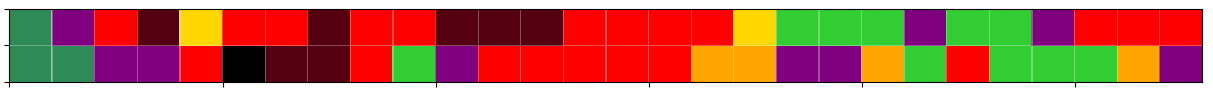
\includegraphics[width=\linewidth,keepaspectratio]{img/two_genomes.png}
  \caption{Graphical representation of document clause genomes}
  \label{fig:docclausegenome}
 \end{center}
 \end{figure}

\patentParagraph Vectorization:
Instead of the original text, just the genome strings now represent the documents. This new content then used to vectorize by Tf-Idf as shown in Fig. \ref{genomevectors}.

 \begin{figure}[h!]
 \begin{center}
  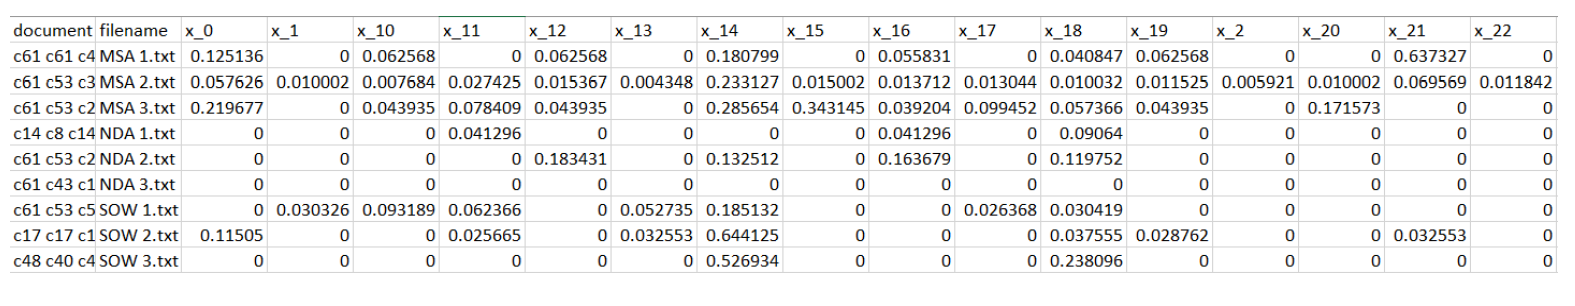
\includegraphics[width=\linewidth]{img/genomevectors.png}
  \caption{Vector representation of document clause genomes}
  \label{fig:genomevectors}
 \end{center}
 \end{figure}

\patentParagraph Vectorization:
Instead of the original text, just the genome strings now represent the documents. This new content then used to vectorize by Tf-Idf as shown in Fig. \ref{genomevectors}.

 \begin{figure}[h!]
 \begin{center}
  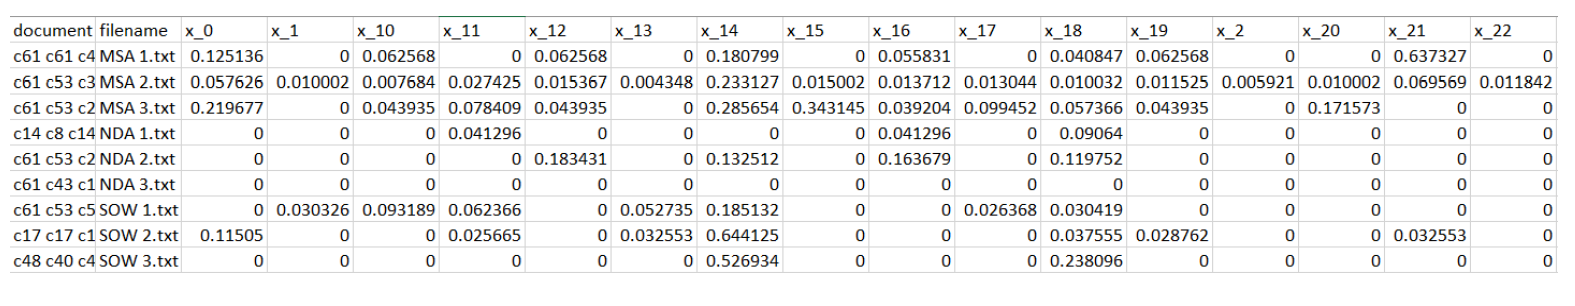
\includegraphics[width=\linewidth]{img/genomevectors.png}
  \caption{Vector representation of document clause genomes}
  \label{fig:genomevectors}
 \end{center}
 \end{figure}
 
 Efficacy of the `Clause Genome' based approach for Similarity calculations can be demonstrated by checking two Master Service Agreements (MSA) and then checking between one MSA and one NDA (Non-Disclosure Agreement). Results are:

 \begin{itemize}
 \item Cosine Similarity: MSA 1 and MSA 2: 0.734940271290997 
\item Cosine Similarity: MSA 1 and NDA 1: 0.31642358837691426 
\end{itemize}

It can be clearly seen that the similar type of documents has high and dissimilar ones have low similarity score. Meaning, clause genome
representation is quantitatively in agreement with the document language


\patentClaimsStart

\beginClaim{Claim1}

Contract documents can be effectlvely representated by their clause category labels, known as ``clause genome''.

\beginClaim{Claim2}

``Clause Genome'' effectiveness is proven in case of contracts similarity assessment.

\patentClaimsEnd

\patentSection{Abstract}

Contracts drive large scale commercial transactions. Being a legal document, it is binding to all the parties, stakeholders involved. Composition contracts using clauses in an unambiguous manner is key to a good contract design. Contract analysis becomes critical in case of already drafted contract for detecting important clauses, obligations, key attributes, etc. Artificial Intelligence, in form of Machine Learning is being used effectively in some of these critical requirements. Finding similar contracts, grouping them is one such specific example.

Text needs to be converted to numbers to be used for Machine Learning applications. Various such vectorization techniques are available, which are primarily statistical in nature and deal with words in the documents. Word vectors are then composed into respective document vectors. This paper proposes vectorization of a higher-level abstraction, called clauses, there by bringing domain specific semantic composition into vectorization. Efficacy of the proposed approach has been demonstrated using Similarity and Clustering algorithms.

\patentDrawings

\bibliographystyle{plain}
\bibliography{References}
\end{document}
